\documentclass{article}
\usepackage{fullpage}
\usepackage{amsmath}
\usepackage{amssymb}
\usepackage{xfrac}
\usepackage{multirow}

% Schreibweisen für bestimmte Überschriften:
%
%					Beispiele
% \section{große Überschrift} 		Folgen und Reihen
% \subsection{große Überschrift} 	Häufungspunkte und Grenzwerte von Folgen
% \paragraph{Definition}
% \paragraph{Schreibweise}
% \paragraph{Bemerkung}
% \paragraph{Bezeichnung}
% \paragraph{Satz}

\begin{document}
% start
\paragraph{Bsp}
\begin{align*}
	f(x)&=x^3 , \ x \in \mathbb{R}^3 
	\\
	f'(x)&=3x^2
	\\	
	f''(x)&=6x \left\{ 
		\begin{array}{c} 
			> 0, \ x > 0
			\\
			< 0, \ x < 0
		\end{array} 
	\right.
\end{align*}
\begin{center}
	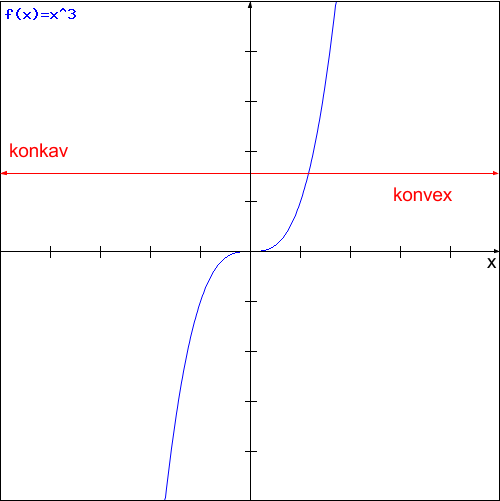
\includegraphics[scale=0.5]{png/konkav_konvex.png}
\end{center}
\paragraph{Bsp} 
In welchen Intervallen des Definitionsbereichs ist die Funktion f
\\
a) \quad monoton steigend bzw. fallend \\
b) \quad konvex bzw. konkav?
\begin{align*}
	f(x)=\frac{x-3}{x^2}, D_f&=\mathbb{R} \backslash\{0\}
	\\
	&=(-\infty, 0)\cup(0,\infty)
\end{align*}
\begin{align*}
	\text{a)} \quad f'(x)=&\frac{(x-3)'x^2-(x-3)(x^2)'}{(x^2)^2}
	\\
	=&\frac{1 \cdot{x^2}-(x-3) \cdot{2x}}{x^4}
	\\
	=&\frac{x[x-2(x-3)]}{x^4}
	\\
	=&\frac{6-x}{x^3}
	\\
	\\
	f'(x) = 0 \quad \text{f\"ur} \ x = 6  
\end{align*}
Dem Zwischenwertsatz zufolge hat eine in einem Intervall stetige Funktion,
die dort keine Nullstellen besitzt, im gesamten Intervall das selbe Vorzeichen.
\begin{align*}
	I_1&=(-\infty,0):x=-1 \in I_1,f'(-1)=-7 < 0
	\\
	I_2&=(0,6):f'(1)=5 > 0
	\\
	I_3&=(6,\infty):f'(7)=-\frac{1}{7^3} < 0	
\end{align*}
\begin{align*}
	f'(x) < 0 \ \forall x \in I_1
	\\
	f \ \text{ist streng monoton fallend in} \ I_1
	\\	
	f'(x) > 0 \ \forall x \in I_2
	\\
	f \ \text{ist streng monoton wachsend in} \ I_2
	\\	
	f'(x) < 0 \ \forall x \in I_3
	\\
	f \ \text{ist streng monoton fallend in} \ I_3
\end{align*}
\begin{center}
	
\includegraphics[scale=0.5]{png/intervall_nullstellen.png}
\end{center}
% stop

\end{document}
